\documentclass[12pt]{article}
\usepackage{hyperref}
\usepackage{pdflscape}
\usepackage{longtable}
\usepackage{graphicx}
\usepackage{tabularx}
\usepackage{booktabs}
\graphicspath{ {.} }
\usepackage{times} % or \usepackage{mathptmx} for Times + math
\usepackage[margin=0.8in]{geometry}


\title{Proposal and Contract for 4AL3 ML Project}
\author{Rebecca Di Filippo, Jake Read, Claire Nielsen}
\date{\today}


\begin{document}

\maketitle

\newpage
\section{Team Members}

\textbf{Rebecca Di Filippo}\\
difilir@mcmaster.ca\\

\textbf{Jake Read}\\
readj9@mcmaster.ca\\

\textbf{Claire Nielsen}\\
nielsc2@mcmaster.ca\\

\section{Task Title and Overview}
\textbf{Task Title:} Asteroid Classification Using Machine Learning \newline

\textbf{Overview:} 
This project aims to classify asteroids based on their orbital and physical characteristics to predict potentially hazardous asteroids (PHAs) versus non-hazardous ones. 
Accurate classification of asteroids is crucial for early warning systems, space mission planning, and planetary defense. \newline

\textbf{Significance:}
\begin{itemize}
    \item Helps analyze the potential threat various asteroids pose to Earth.
    \item Provides insights into asteroid characteristics for scientific and space exploration purposes.
\end{itemize}

\textbf{Challenges:}
\begin{itemize}
    \item Class imbalance: less hazardous asteroids in the set, which may affect model performance.
    \item Some features may be correlated or redundant which requires feature selection techniques.
    \item Some fields are missing, and may need to be approximated based on other features.
    \item Complex features without clear meaning, that we will have to research to understand.
\end{itemize}

\section{Task Definition}
\begin{itemize}
    \item \textbf{Type of Data:} Structured dataset with numerical features (orbital parameters, size) and categorical labels (hazardous vs. non-hazardous).
    \item \textbf{Task Type:} Supervised classification.
    \item \textbf{Number of Classes:} 2 (Potentially Hazardous, Non-Hazardous)
    \item \textbf{Input:} Chosen features from data set
    \item \textbf{Output:} \texttt{pha} (Potentially Hazardous Asteroid flag — the classification label to be predicted)
    \item \textbf{Label Type:} Single-label (asteroid is either potentially hazardous or not).
\end{itemize}

\section{Problem Description}
Asteroids pose a threat to Earth.
While most asteroids orbit safely, some come close enough to be considered potentially hazardous and could cause significant damage if they were to impact Earth.
Predicting which asteroids are hazardous allows space agencies to prioritize observation on certain asteroids, develop mitigation strategies, and design early-warning systems.
The classification of asteroids is difficult and time-consuming work, requiring analysis of a large variety of aspects about a given asteroid.
As such, a model capable of predicting such data would be a great boon.

\section{Data Sources and Plan for Data Collection / Labeling}

\textbf{Data Source and Description:}

The dataset is publicly available on Kaggle under the name \textit{Asteroid Dataset} by user \textit{sakhawat18}.
It is derived from NASA and JPL’s Small-Body and Asteroid databases, containing both orbital and physical properties for hundreds of thousands of known asteroids.
The dataset includes 45 features, as follows:

\begin{itemize}
    \item \textbf{Identifiers and Metadata:} \texttt{id}, \texttt{spkid}, \texttt{full\_name}, \texttt{pdes}, \texttt{name}, \texttt{prefix}, \texttt{orbit\_id}, \texttt{class}

    \item \textbf{Flags:} \texttt{neo} (Near-Earth Object flag), \texttt{pha} (Potentially Hazardous Asteroid flag, 1 = hazardous, 0 = non-hazardous)

    \item \textbf{Physical Properties:} \texttt{H} (absolute magnitude), \texttt{diameter} (km), \texttt{albedo} (surface reflectivity), \texttt{diameter\_sigma} (uncertainty in diameter)

    \item \textbf{Orbital Elements:}
    \begin{itemize}
        \item Core orbital parameters: \texttt{e} (eccentricity), \texttt{a} (semi-major axis), \texttt{q} (perihelion distance), \texttt{i} (inclination), \texttt{om} ($\Omega$, longitude of ascending node), \texttt{w} ($\omega$, argument of perihelion), \texttt{ma} (mean anomaly)
        \item Derived orbital distances: \texttt{ad} (aphelion distance), \texttt{moid} (minimum orbit intersection distance), \texttt{moid\_ld} (MOID in lunar distances)
        \item Motion and timing: \texttt{n} (mean motion), \texttt{tp} (time of perihelion passage), \texttt{per} (orbital period in days), \texttt{per\_y} (orbital period in years)
    \end{itemize}

    \item \textbf{Epoch and Reference Data:} \texttt{epoch}, \texttt{epoch\_mjd} (Modified Julian Date), \texttt{epoch\_cal} (calendar format), \texttt{equinox}, \texttt{tp\_cal} (perihelion passage in calendar format)

    \item \textbf{Uncertainties (Standard Deviations):} \texttt{sigma\_e}, \texttt{sigma\_a}, \texttt{sigma\_q}, \texttt{sigma\_i}, \texttt{sigma\_om}, \texttt{sigma\_w}, \texttt{sigma\_ma}, \texttt{sigma\_ad}, \texttt{sigma\_n}, \texttt{sigma\_tp}, \texttt{sigma\_per}

    \item \textbf{Model Fit Quality:} \texttt{rms} (root-mean-square residual, indicating fit accuracy of the orbital solution)

    \item \textbf{Target Label:} \texttt{pha} (Potentially Hazardous Asteroid flag — the classification label to be predicted)
\end{itemize}

\textbf{Data Handling Plan:}
\begin{enumerate}
    \item \textbf{Collection:} We will download the dataset directly from Kaggle using the Kaggle API, complying with its terms of service.
    \item \textbf{Cleaning:}
    \begin{itemize}
        \item Inspect and handle missing values (e.g., impute or drop based on completeness).
        \item Remove identifier columns that do not provide predictive value.
        \item Normalize continuous variables to consistent ranges.
    \end{itemize}
    \item \textbf{Feature Engineering:}
    \begin{itemize}
        \item We plan to experiment with various feature sets. We will begin by experimenting with more obvious features, such as those related to physical properties, and then over time add more features until we're using the entire dataset if that gives the best results.
        \item Potentially apply dimensionality reduction (PCA) or correlation-based feature selection.
    \end{itemize}
    \item \textbf{Label Verification:}
    The dataset includes a binary label \texttt{PHA}, so no manual labeling is required. We will validate the class balance and ensure consistent encoding.
    \item \textbf{Imbalance Handling:}
    Because the hazardous class is rare, we will address class imbalance through oversampling (e.g., SMOTE), undersampling, or weighted loss functions during model training.
\end{enumerate}

\textbf{Subset Use:}
If the dataset is too large for efficient prototyping, we may initially work with a random balanced subset, then scale to the full dataset for final training and evaluation. \newline

\textbf{Metadata:}
We will document all preprocessing decisions, including dropped columns, imputation methods, and feature transformations. \newline

\textbf{Sources:}
\begin{itemize}
    \item Kaggle source: \url{https://www.kaggle.com/datasets/sakhawat18/asteroid-dataset}
    \item Original source: \url{https://ssd.jpl.nasa.gov/tools/sbdb_query.html}
\end{itemize}


\section{Dataset Sample}
The full dataset has just under one million data points.
A sample of the first 3 rows can be seen below.
Only the first 10 columns are shown, as there are too many features to fit in the document otherwise:

% \begin{landscape}
\begin{scriptsize}
\begin{longtable}{|c|c|c|c|c|c|c|c|c|c|}
\caption{First 3 rows of the asteroid dataset (truncated for readability)} \\
\hline
\textbf{id} & \textbf{spkid} & \textbf{full\_name} & \textbf{pdes} & \textbf{name} & \textbf{neo} & \textbf{pha} & \textbf{H} & \textbf{diameter} & \textbf{albedo} \\
\hline
\endfirsthead
\hline
\textbf{id} & \textbf{spkid} & \textbf{full\_name} & \textbf{pdes} & \textbf{name} & \textbf{neo} & \textbf{pha} & \textbf{H} & \textbf{diameter} & \textbf{albedo} \\
\hline
\endhead
a0000001 & 2000001 & 1 Ceres & 1 & Ceres & N & N & 3.4 & 939.4 & 0.09 \\
\hline
a0000002 & 2000002 & 2 Pallas & 2 & Pallas & N & N & 4.2 & 545 & 0.101 \\
\hline
a0000003 & 2000003 & 3 Juno & 3 & Juno & N & N & 5.33 & 246.596 & 0.214 \\
\hline
\end{longtable}
\end{scriptsize}
% \end{landscape}
\section{Proposed Solution}

\subsection*{How we plan to go about solving this problem?}
\medskip
Although we haven’t been explicitly taught tree-based ensemble methods yet,
this approach uses ideas from class such as supervised learning, classification,
model training, and evaluation. We will build a system that
cleans and preprocesses the asteroid dataset, selects and engineers relevant
features, and trains a model using machine learning to classify asteroids as potentially hazardous
or not. We will handle class imbalance using techniques like oversampling( e.g., SMOTE)),
or weighted loss, and then evaluate the model.



\medskip

% What kind of features and target labels do you have?
\subsection*{Features and Target Labels}
\medskip
\textbf{Target label:} \texttt{pha} — binary (1 = potentially hazardous, 0 = non-hazardous). \\
\textbf{Features:} 
\begin{itemize}
    \item \textbf{Physical Properties:} \texttt{H} (absolute magnitude), \texttt{diameter} (km), \texttt{albedo} (surface reflectivity), \texttt{diameter\_sigma} (uncertainty in diameter)

    \item \textbf{Orbital Elements:}
    \begin{itemize}
        \item Core orbital parameters: \texttt{e} (eccentricity), \texttt{a} (semi-major axis), \texttt{q} (perihelion distance), \texttt{i} (inclination), \texttt{om} ($\Omega$, longitude of ascending node), \texttt{w} ($\omega$, argument of perihelion), \texttt{ma} (mean anomaly)
        \item Derived orbital distances: \texttt{ad} (aphelion distance), \texttt{moid} (minimum orbit intersection distance), \texttt{moid\_ld} (MOID in lunar distances)
        \item Motion and timing: \texttt{n} (mean motion), \texttt{tp} (time of perihelion passage), \texttt{per} (orbital period in days), \texttt{per\_y} (orbital period in years)
    \end{itemize}

    \item \textbf{Uncertainties (Standard Deviations):} \texttt{sigma\_e}, \texttt{sigma\_a}, \texttt{sigma\_q}, \texttt{sigma\_i}, \texttt{sigma\_om}, \texttt{sigma\_w}, \texttt{sigma\_ma}, \texttt{sigma\_ad}, \texttt{sigma\_n}, \texttt{sigma\_tp}, \texttt{sigma\_per}

    \item \textbf{Model Fit Quality:} \texttt{rms} (root-mean-square residual, indicating fit accuracy of the orbital solution)

\end{itemize}

The left out features are identifiers, metadata, epoch and reference data, that do not contribute to prediction.
\medskip

\emph{NOTE:We may also create derived features combining orbital and physical properties if needed.}


\subsection*{Models}
\begin{itemize}
    \item \textbf{Favoured Approach:} Gradient Boosted Trees because from research it seems like they handle structured tabular data well, manage non-linear relationships, and allow weighting for class imbalance.

    \item \textbf{Alternative models:} Random Forests, or Neural Networks are worth considering if gradient boosting does not yield good results.
    
\end{itemize}

\subsection*{Existing Solutions}
\medskip
There exists several deep learning-assisted models of Near Earth Asteroid (NEA) tracking programs. One noted model is described in \textit{Deep learning-assisted near-Earth asteroid tracking in astronomical images}. It focuses on NEA tracking through images. Deep learning has made remarkable strides in tracking through image detection, however neural network training has remained a challenge due to a lack of sufficient data (Du et al., 2024). \\

It has also been noted by Sykes et al. (2000) that gradient boosting can provide an accurate detection and classification model based on asteroid features. The team's goal is to produce an accurate model using that strategy. 

\subsection*{Evaluation on Correctness of Model}

The team will evaluate the performance of the model based on the existing PHA flag that notes whether or not the NEA is hazardous. By training the model on features that can be markers that an asteroid is hazardous, the model should correctly identify hazardous NEAs to within 20\% absolute error using the data that already exists. It is important to note that since there is a class imbalance and hazardous classes are quite rare, this qualifier is less stable. 

\subsection*{Libraries/Tools}
Listed are libraries the team intends to use for the project, and their intended purposes. \\
\textbf{Computation}
\begin{itemize}
    \item pandas, for data manipulation and analysis
    \item numpy, for numerical computations
    \item scikit-learn, for preprocessing, feature selection, and machine learning models
\end{itemize}

\textbf{Machine Learning}
\begin{itemize}
    \item imbalanced-learn, for handling class imbalance in the data
    \item xgboost, for implemented gradient-boosted trees
    \item lightgbm,as an alternative to xgboost
    \item catboost, as an alternative to xboost that can specialize in categorical data
\end{itemize}

\textbf{Visualization}
\begin{itemize}
    \item matplotlib, for creating static plots
    \item seaborn, for static data visualization
    \item plotly, for interactive visualizations
\end{itemize}

\textbf{Evaluation}
\begin{itemize}
    \item scikit-learn, for metrics such as classification reports, confusion matrices, and Receiver Operating Characteristic (ROC) curves
\end{itemize}

\textbf{Notebook Support}
\begin{itemize}
    \item jupyter, for running jupyter notebooks for exploratory data analysis (EDA)
\end{itemize}

\subsection*{Sources/References}

Du, Z., Jiang, H., Yang, X., Cheng, H., \& Liu, J. (2024). Deep learning-assisted near-Earth asteroid tracking in astronomical images. \textit{Advances in Space Research}, 73(10), 5349–5362. https://doi.org/10.1016/j.asr.2024.02.04\\

Khalil, M., Said, M., Sedfy, S. E., Ahmed, A., Khaled, M., Abdellah, N., \& Khaled, N. (2023). Detecting Asteroids and Comets using Machine Learning and Deep Learning. \textit{MSA Engineering Journal, 2(2)}, 967–972. \\ https://doi.org/10.21608/msaeng.2023.291924\\

\medskip

\newpage
\section{Team Charter}
\subsection{Purpose}

Our teams purpose is to create a reasonably accurate model to classify Near Earth Asteroids (NEAs) as hazardous or non-hazardous. Using a Kaggle dataset, the team will train a gradient-boosted tree model to intake asteroid features and use them to classify the NEAs. 

\subsection{Team Member Roles}

The team will rotate to fill several roles throughout the course of the project. The roles are: 

\begin{table}[ht]
\centering
\caption{Non-technical Roles and Descriptions}
\label{tab:non-technical-roles}
\begin{tabularx}{\textwidth}{lX}
\toprule
\textbf{Role} & \textbf{Description} \\
\midrule

Meeting Chair & Prepares meeting agenda or discussion points ahead of time. Facilitates team discussions during the meeting to ensure all required points are addressed. When required, leads delegation of workload.  \\ \\
Team Liaison & Acts as the main point of contact between the team and supervisors and/or stakeholders.  \\ \\
Note Taker & Records meeting minutes. \\ \\
\bottomrule
\end{tabularx}
\end{table}

The team will assign workload based on even delegation of work, as well as personal expertise or comfort in specific areas of the project. Each member will fill a technical role of developer. \\

\subsection{Leadership}

The team will delegate and divide workflow as a collaborative discussion. The Meeting Chair may direct the conversation but all members of the team hold equal decision making power. In the event of an impasse a vote will be held between members; in the event of a stalemate the team will seek advice from peers. \\

\subsection{Meeting Plan}

The team will meet once a week on Thursdays at 3:30pm. Depending on impending workload or deliverables, the team may choose to meet additional times, subject to members' availability. If any member has a conflict with the usual meeting slot, an alternate time may be chosen

\subsection{Communication Plan}

The team will communicate primarily using a discord chat. The chat will be used to communicate over text as well as meeting calls. Any correspondence with a TA should be done over Outlook or Teams. \\

All teammates will endeavor to attend every scheduled meeting. Should the team unanimously decide a meeting is not required, it may be canceled ahead of time. If a teammate is not able to attend a scheduled meeting, they must provide the others with notice in advance, as early as possible and up to twenty-four hours in advance barring emergency circumstances. Permissible emergency circumstances include but are not limited to: \\

\begin{itemize}
    \item Medical concern (migraine, illness, etc.)
    \item Family emergency
    \item Unforseen transit issues \\
\end{itemize}

The same list of circumstances applies should a teammate be responsible for the team missing a deliverable deadline. If a deadline is missed, the team will discuss how to avoid the situation by next scheduled meeting latest. \\

\newpage

\textbf{Team Charter Signatures}\\


\includegraphics[width=0.3\textwidth]{signature_becca}\\
Rebecca Di Filippo \\ 
\date{\today}\\ \\ \\ 

image here\\
Jake Read\\
\date{\today }\\ \\ \\ 

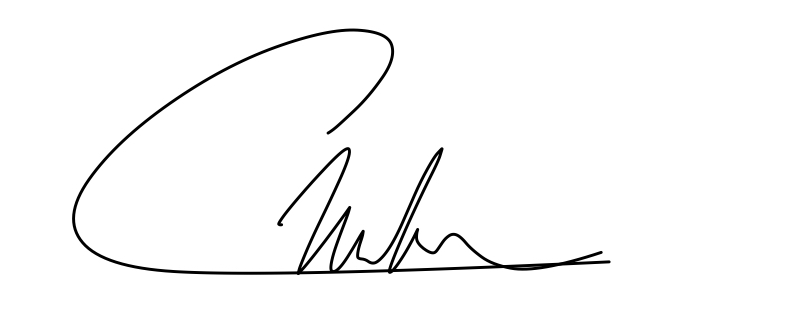
\includegraphics[width=0.3\textwidth]{signature_claire}\\
Claire Nielsen\\
\date{\today}

\end{document}
